
\begin{DoxyItemize}
\item \hyperlink{transforms_eig}{E\-I\-G Eigendecomposition of a Matrix}  
\item \hyperlink{transforms_fft}{F\-F\-T (Inverse) Fast Fourier Transform Function}  
\item \hyperlink{transforms_fftn}{F\-F\-T\-N N-\/\-Dimensional Forward F\-F\-T }  
\item \hyperlink{transforms_fftshift}{F\-F\-T\-S\-H\-I\-F\-T Shift F\-F\-T Output}  
\item \hyperlink{transforms_hilbert}{H\-I\-L\-B\-E\-R\-T Hilbert Transform}  
\item \hyperlink{transforms_ifftn}{I\-F\-F\-T\-N N-\/\-Dimensional Inverse F\-F\-T }  
\item \hyperlink{transforms_ifftshift}{I\-F\-F\-T\-S\-H\-I\-F\-T Inverse Shift F\-F\-T Output}  
\item \hyperlink{transforms_inv}{I\-N\-V Invert Matrix}  
\item \hyperlink{transforms_lu}{L\-U L\-U Decomposition for Matrices}  
\item \hyperlink{transforms_qr}{Q\-R Q\-R Decomposition of a Matrix}  
\item \hyperlink{transforms_svd}{S\-V\-D Singular Value Decomposition of a Matrix}  
\end{DoxyItemize}\hypertarget{transforms_eig}{}\section{E\-I\-G Eigendecomposition of a Matrix}\label{transforms_eig}
Section\-: \hyperlink{sec_transforms}{Transforms/\-Decompositions} \hypertarget{vtkwidgets_vtkxyplotwidget_Usage}{}\subsection{Usage}\label{vtkwidgets_vtkxyplotwidget_Usage}
Computes the eigendecomposition of a square matrix. The {\ttfamily eig} function has several forms. The first returns only the eigenvalues of the matrix\-: \begin{DoxyVerb}  s = eig(A)
\end{DoxyVerb}
 The second form returns both the eigenvectors and eigenvalues as two matrices (the eigenvalues are stored in a diagonal matrix)\-: \begin{DoxyVerb}  [V,D] = eig(A)
\end{DoxyVerb}
 where {\ttfamily D} is the diagonal matrix of eigenvalues, and {\ttfamily V} is the matrix of eigenvectors.

Eigenvalues and eigenvectors for asymmetric matrices {\ttfamily A} normally are computed with balancing applied. Balancing is a scaling step that normaly improves the quality of the eigenvalues and eigenvectors. In some instances (see the Function Internals section for more details) it is necessary to disable balancing. For these cases, two additional forms of {\ttfamily eig} are available\-: \begin{DoxyVerb}  s = eig(A,'nobalance'),
\end{DoxyVerb}
 which computes the eigenvalues of {\ttfamily A} only, and does not balance the matrix prior to computation. Similarly, \begin{DoxyVerb}  [V,D] = eig(A,'nobalance')
\end{DoxyVerb}
 recovers both the eigenvectors and eigenvalues of {\ttfamily A} without balancing. Note that the 'nobalance' option has no affect on symmetric matrices.

Free\-Mat also provides the ability to calculate generalized eigenvalues and eigenvectors. Similarly to the regular case, there are two forms for {\ttfamily eig} when computing generalized eigenvector (see the Function Internals section for a description of what a generalized eigenvector is). The first returns only the generalized eigenvalues of the matrix pair {\ttfamily A,B} \begin{DoxyVerb}  s = eig(A,B)
\end{DoxyVerb}
 The second form also computes the generalized eigenvectors, and is accessible via \begin{DoxyVerb}  [V,D] = eig(A,B)
\end{DoxyVerb}
 \hypertarget{transforms_svd_Function}{}\subsection{Internals}\label{transforms_svd_Function}
Recall that {\ttfamily v} is an eigenvector of {\ttfamily A} with associated eigenvalue {\ttfamily d} if \[ A v = d v. \] This decomposition can be written in matrix form as \[ A V = V D \] where \[ V = [v_1,v_2,\ldots,v_n], D = \mathrm{diag}(d_1,d_2,\ldots,d_n). \] The {\ttfamily eig} function uses the {\ttfamily L\-A\-P\-A\-C\-K} class of functions {\ttfamily G\-E\-E\-V\-X} to compute the eigenvalue decomposition for non-\/symmetric (or non-\/\-Hermitian) matrices {\ttfamily A}. For symmetric matrices, {\ttfamily S\-S\-Y\-E\-V} and {\ttfamily D\-S\-Y\-E\-V} are used for {\ttfamily float} and {\ttfamily double} matrices (respectively). For Hermitian matrices, {\ttfamily C\-H\-E\-E\-V} and {\ttfamily Z\-H\-E\-E\-V} are used for {\ttfamily complex} and {\ttfamily dcomplex} matrices.

For some matrices, the process of balancing (in which the rows and columns of the matrix are pre-\/scaled to facilitate the search for eigenvalues) is detrimental to the quality of the final solution. This is particularly true if the matrix contains some elements on the order of round off error. See the Example section for an example.

A generalized eigenvector of the matrix pair {\ttfamily A,B} is simply a vector {\ttfamily v} with associated eigenvalue {\ttfamily d} such that \[ A v = d B v, \] where {\ttfamily B} is a square matrix of the same size as {\ttfamily A}. This decomposition can be written in matrix form as \[ A V = B V D \] where \[ V = [v_1,v_2,\ldots,v_n], D = \mathrm{diag}(d_1,d_2,\ldots,d_n). \] For general matrices {\ttfamily A} and {\ttfamily B}, the {\ttfamily G\-G\-E\-V} class of routines are used to compute the generalized eigendecomposition. If howevever, {\ttfamily A} and {\ttfamily B} are both symmetric (or Hermitian, as appropriate), Then Free\-Mat first attempts to use {\ttfamily S\-S\-Y\-G\-V} and {\ttfamily D\-S\-Y\-G\-V} for {\ttfamily float} and {\ttfamily double} arguments and {\ttfamily C\-H\-E\-G\-V} and {\ttfamily Z\-H\-E\-G\-V} for {\ttfamily complex} and {\ttfamily dcomplex} arguments (respectively). These routines requires that {\ttfamily B} also be positive definite, and if it fails to be, Free\-Mat will revert to the routines used for general arguments. \hypertarget{variables_struct_Example}{}\subsection{Example}\label{variables_struct_Example}
Some examples of eigenvalue decompositions. First, for a diagonal matrix, the eigenvalues are the diagonal elements of the matrix.


\begin{DoxyVerbInclude}
--> A = diag([1.02f,3.04f,1.53f])

A = 
    1.0200         0         0 
         0    3.0400         0 
         0         0    1.5300 

--> eig(A)

ans = 
    1.0200 
    1.5300 
    3.0400 
\end{DoxyVerbInclude}


Next, we compute the eigenvalues of an upper triangular matrix, where the eigenvalues are again the diagonal elements.


\begin{DoxyVerbInclude}
--> A = [1.0f,3.0f,4.0f;0,2.0f,6.7f;0.0f,0.0f,1.0f]

A = 
    1.0000    3.0000    4.0000 
         0    2.0000    6.7000 
         0         0    1.0000 

--> eig(A)

ans = 
 1 
 2 
 1 
\end{DoxyVerbInclude}


Next, we compute the complete eigenvalue decomposition of a random matrix, and then demonstrate the accuracy of the solution


\begin{DoxyVerbInclude}
--> A = float(randn(2))

A = 
    0.3747   -1.5129 
   -0.6283   -1.1096 

--> [V,D] = eig(A)
V = 
    0.9526    0.6096 
   -0.3042    0.7927 

D = 
    0.8578         0 
         0   -1.5928 

--> A*V - V*D

ans = 

   1.0e-08 * 
   -5.9605         0 
   -2.9802         0 
\end{DoxyVerbInclude}


Now, we consider a matrix that requires the nobalance option to compute the eigenvalues and eigenvectors properly. Here is an example from M\-A\-T\-L\-A\-B's manual.


\begin{DoxyVerbInclude}
--> B = [3,-2,-.9,2*eps;-2,4,1,-eps;-eps/4,eps/2,-1,0;-.5,-.5,.1,1]

B = 
    3.0000   -2.0000   -0.9000    0.0000 
   -2.0000    4.0000    1.0000   -0.0000 
   -0.0000    0.0000   -1.0000         0 
   -0.5000   -0.5000    0.1000    1.0000 

--> [VB,DB] = eig(B)
VB = 
    0.6153   -0.4176   -0.0000   -0.1495 
   -0.7881   -0.3261   -0.0000    0.1316 
   -0.0000   -0.0000    0.0000   -0.9570 
    0.0189    0.8481    1.0000   -0.2110 

DB = 
    5.5616         0         0         0 
         0    1.4384         0         0 
         0         0    1.0000         0 
         0         0         0   -1.0000 

--> B*VB - VB*DB

ans = 
         0         0    0.0000   -0.0000 
         0    0.0000   -0.0000    0.0000 
   -0.0000   -0.0000   -0.0000   -0.0000 
    0.0000    0.0000    0.0000   -0.5088 

--> [VN,DN] = eig(B,'nobalance')
VN = 
    0.6153   -0.4176   -0.0000   -0.1528 
   -0.7881   -0.3261         0    0.1345 
   -0.0000   -0.0000   -0.0000   -0.9781 
    0.0189    0.8481   -1.0000    0.0443 

DN = 
    5.5616         0         0         0 
         0    1.4384         0         0 
         0         0    1.0000         0 
         0         0         0   -1.0000 

--> B*VN - VN*DN

ans = 

   1.0e-15 * 
   -1.7764   -0.1110   -0.5587   -0.1665 
    3.5527    1.0547    0.3364   -0.1943 
    0.0172    0.0015    0.0066         0 
    0.1527   -0.2220    0.2220    0.0833 
\end{DoxyVerbInclude}
 \hypertarget{transforms_fft}{}\section{F\-F\-T (Inverse) Fast Fourier Transform Function}\label{transforms_fft}
Section\-: \hyperlink{sec_transforms}{Transforms/\-Decompositions} \hypertarget{vtkwidgets_vtkxyplotwidget_Usage}{}\subsection{Usage}\label{vtkwidgets_vtkxyplotwidget_Usage}
Computes the Discrete Fourier Transform (D\-F\-T) of a vector using the Fast Fourier Transform technique. The general syntax for its use is \begin{DoxyVerb}  y = fft(x,n,d)
\end{DoxyVerb}
 where {\ttfamily x} is an {\ttfamily n}-\/dimensional array of numerical type. Integer types are promoted to the {\ttfamily double} type prior to calculation of the D\-F\-T. The argument {\ttfamily n} is the length of the F\-F\-T, and {\ttfamily d} is the dimension along which to take the D\-F\-T. If $|$n$|$ is larger than the length of {\ttfamily x} along dimension {\ttfamily d}, then {\ttfamily x} is zero-\/padded (by appending zeros) prior to calculation of the D\-F\-T. If {\ttfamily n} is smaller than the length of {\ttfamily x} along the given dimension, then {\ttfamily x} is truncated (by removing elements at the end) to length {\ttfamily n}.

If {\ttfamily d} is omitted, then the D\-F\-T is taken along the first non-\/singleton dimension of {\ttfamily x}. If {\ttfamily n} is omitted, then the D\-F\-T length is chosen to match of the length of {\ttfamily x} along dimension {\ttfamily d}.

Note that F\-F\-T support on Linux builds requires availability of the F\-F\-T\-W libraries at compile time. On Windows and Mac O\-S X, single and double precision F\-F\-Ts are available by default. \hypertarget{transforms_svd_Function}{}\subsection{Internals}\label{transforms_svd_Function}
The output is computed via \[ y(m_1,\ldots,m_{d-1},l,m_{d+1},\ldots,m_{p}) = \sum_{k=1}^{n} x(m_1,\ldots,m_{d-1},k,m_{d+1},\ldots,m_{p}) e^{-\frac{2\pi(k-1)l}{n}}. \]

For the inverse D\-F\-T, the calculation is similar, and the arguments have the same meanings as the D\-F\-T\-: \[ y(m_1,\ldots,m_{d-1},l,m_{d+1},\ldots,m_{p}) = \frac{1}{n} \sum_{k=1}^{n} x(m_1,\ldots,m_{d-1},k,m_{d+1},\ldots,m_{p}) e^{\frac{2\pi(k-1)l}{n}}. \] The F\-F\-T is computed using the F\-F\-T\-Pack library, available from netlib at {\ttfamily \href{http://www.netlib.org}{\tt http\-://www.\-netlib.\-org}}. Generally speaking, the computational cost for a F\-F\-T is (in worst case) {\ttfamily O(n$^\wedge$2)}. However, if {\ttfamily n} is composite, and can be factored as \[ n = \prod_{k=1}^{p} m_k, \] then the D\-F\-T can be computed in \[ O(n \sum_{k=1}^{p} m_k) \] operations. If {\ttfamily n} is a power of 2, then the F\-F\-T can be calculated in {\ttfamily O(n log\-\_\-2 n)}. The calculations for the inverse F\-F\-T are identical. \hypertarget{variables_struct_Example}{}\subsection{Example}\label{variables_struct_Example}
The following piece of code plots the F\-F\-T for a sinusoidal signal\-:


\begin{DoxyVerbInclude}
--> t = linspace(0,2*pi,128);
--> x = cos(15*t);
--> y = fft(x);
--> plot(t,abs(y));
\end{DoxyVerbInclude}


The resulting plot is\-:  
\begin{DoxyImage}
\includegraphics[width=12cm]{fft1}
\caption{fft1}
\end{DoxyImage}


The F\-F\-T can also be taken along different dimensions, and with padding and/or truncation. The following example demonstrates the Fourier Transform being computed along each column, and then along each row.


\begin{DoxyVerbInclude}
--> A = [2,5;3,6]

A = 
 2 5 
 3 6 

--> real(fft(A,[],1))

ans = 
  5 11 
 -1 -1 

--> real(fft(A,[],2))

ans = 
  7 -3 
  9 -3 
\end{DoxyVerbInclude}


Fourier transforms can also be padded using the {\ttfamily n} argument. This pads the signal with zeros prior to taking the Fourier transform. Zero padding in the time domain results in frequency interpolation. The following example demonstrates the F\-F\-T of a pulse (consisting of 10 ones) with (red line) and without (green circles) padding.


\begin{DoxyVerbInclude}
--> delta(1:10) = 1;
--> plot((0:255)/256*pi*2,real(fft(delta,256)),'r-');
--> hold on
--> plot((0:9)/10*pi*2,real(fft(delta)),'go');
\end{DoxyVerbInclude}


The resulting plot is\-:  
\begin{DoxyImage}
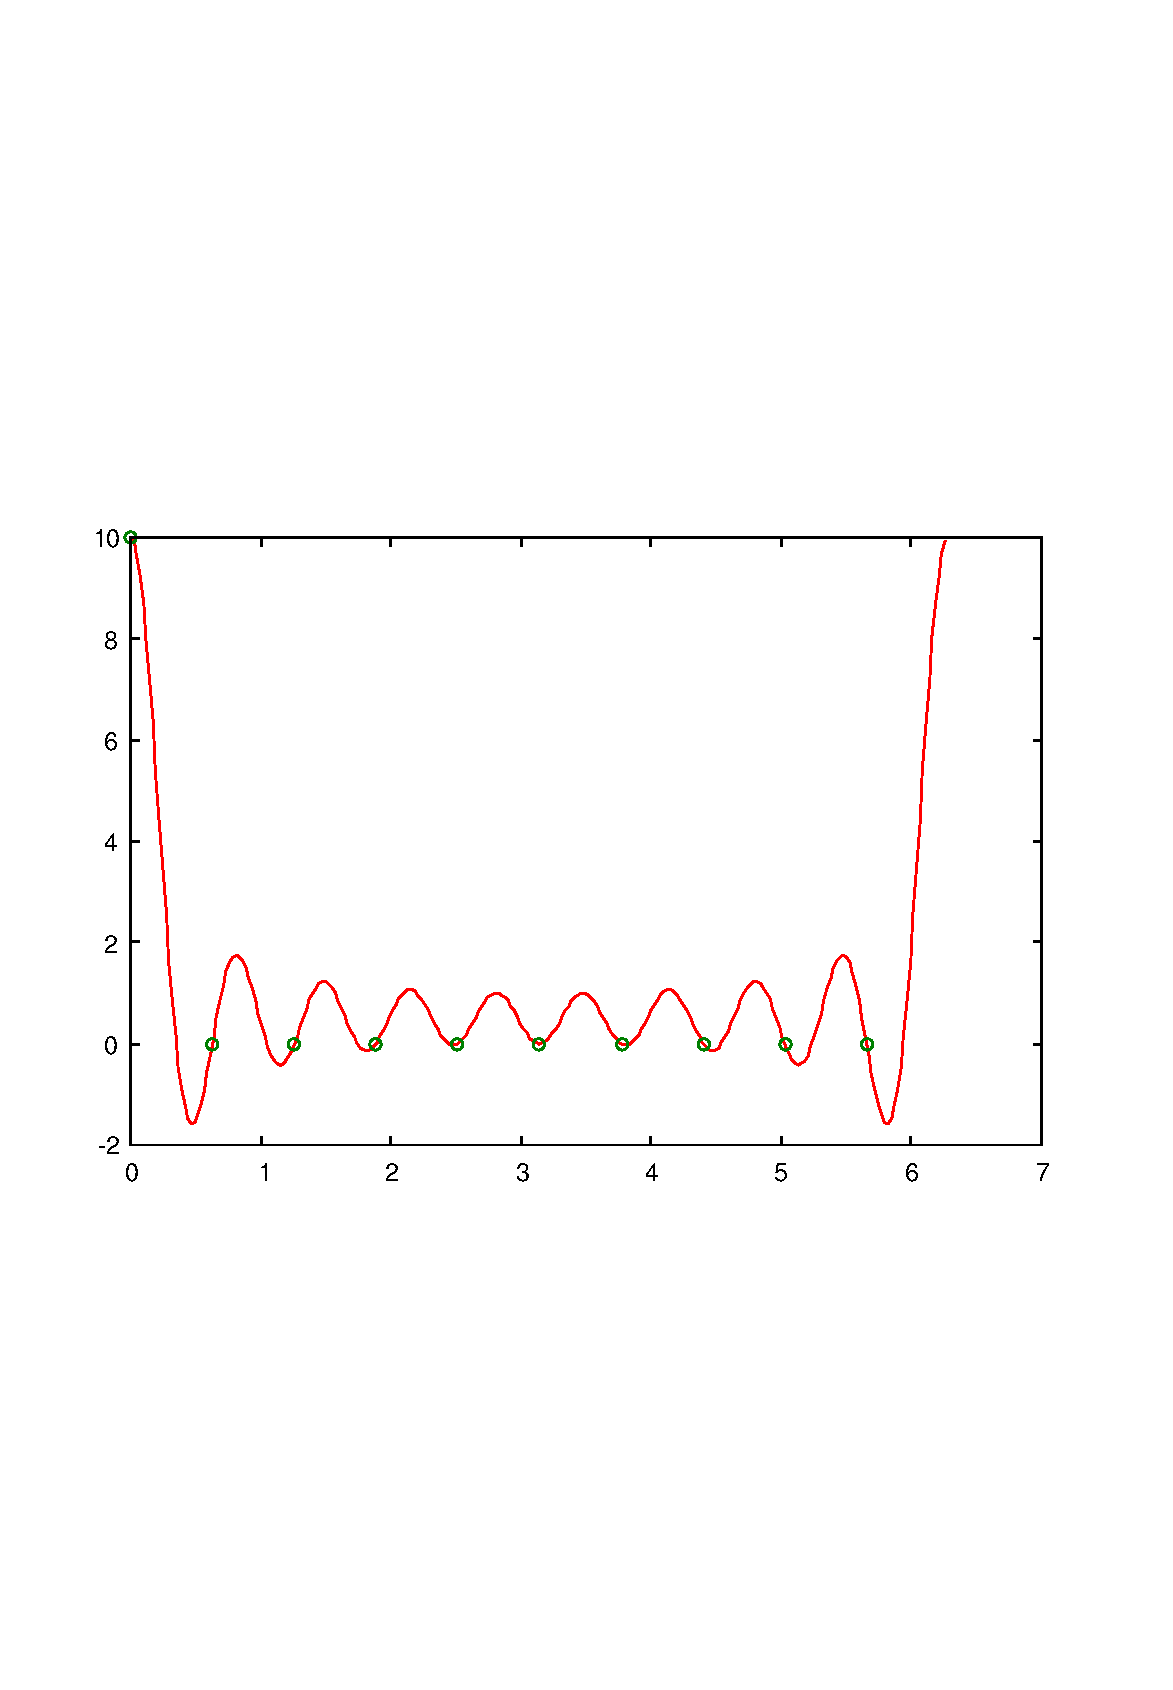
\includegraphics[width=12cm]{fft2}
\caption{fft2}
\end{DoxyImage}
 \hypertarget{transforms_fftn}{}\section{F\-F\-T\-N N-\/\-Dimensional Forward F\-F\-T}\label{transforms_fftn}
Section\-: \hyperlink{sec_transforms}{Transforms/\-Decompositions} \hypertarget{vtkwidgets_vtkxyplotwidget_Usage}{}\subsection{Usage}\label{vtkwidgets_vtkxyplotwidget_Usage}
Computes the D\-F\-T of an N-\/dimensional numerical array along all dimensions. The general syntax for its use is \begin{DoxyVerb}  y = fftn(x)
\end{DoxyVerb}
 which computes the same-\/size F\-F\-Ts for each dimension of {\ttfamily x}. Alternately, you can specify the size vector \begin{DoxyVerb}  y = fftn(x,dims)
\end{DoxyVerb}
 where {\ttfamily dims} is a vector of sizes. The array {\ttfamily x} is zero padded or truncated as necessary in each dimension so that the output is of size {\ttfamily dims}. The {\ttfamily fftn} function is implemented by a sequence of calls to {\ttfamily fft}. \hypertarget{transforms_fftshift}{}\section{F\-F\-T\-S\-H\-I\-F\-T Shift F\-F\-T Output}\label{transforms_fftshift}
Section\-: \hyperlink{sec_transforms}{Transforms/\-Decompositions} \hypertarget{vtkwidgets_vtkxyplotwidget_Usage}{}\subsection{Usage}\label{vtkwidgets_vtkxyplotwidget_Usage}
The {\ttfamily fftshift} function shifts the D\-C component (zero-\/frequency) of the output from an F\-F\-T to the center of the array. For vectors this means swapping the two halves of the vector. For matrices, the first and third quadrants are swapped. So on for N-\/dimensional arrays. The syntax for its use is \begin{DoxyVerb}     y = fftshift(x).
\end{DoxyVerb}
 Alternately, you can specify that only one dimension be shifted \begin{DoxyVerb}     y = fftshift(x,dim).
\end{DoxyVerb}
 \hypertarget{transforms_hilbert}{}\section{H\-I\-L\-B\-E\-R\-T Hilbert Transform}\label{transforms_hilbert}
Section\-: \hyperlink{sec_transforms}{Transforms/\-Decompositions} \hypertarget{vtkwidgets_vtkxyplotwidget_Usage}{}\subsection{Usage}\label{vtkwidgets_vtkxyplotwidget_Usage}
The {\ttfamily hilbert} function computes the hilbert transform of the argument vector or matrix. The Free\-Mat {\ttfamily hilbert} function is compatible with the one from the M\-A\-T\-L\-A\-B A\-P\-I. This means that the output of the {\ttfamily hilbert} function is the sum of the original function and an imaginary signal containing the Hilbert transform of it. There are two syntaxes for the hilbert function. The first is \begin{DoxyVerb}  y = hilbert(x)
\end{DoxyVerb}
 where {\ttfamily x} is real vector or matrix. If {\ttfamily x} is a matrix, then he Hilbert transform is computed along the columns of {\ttfamily x}. The second syntax provides a dimension along which to take the transform. \begin{DoxyVerb}  y = hilbert(x,n)
\end{DoxyVerb}
 where {\ttfamily n} is the dimension along which to apply the transformation. \hypertarget{transforms_ifftn}{}\section{I\-F\-F\-T\-N N-\/\-Dimensional Inverse F\-F\-T}\label{transforms_ifftn}
Section\-: \hyperlink{sec_transforms}{Transforms/\-Decompositions} \hypertarget{vtkwidgets_vtkxyplotwidget_Usage}{}\subsection{Usage}\label{vtkwidgets_vtkxyplotwidget_Usage}
Computes the inverse D\-F\-T of an N-\/dimensional numerical array along all dimensions. The general syntax for its use is \begin{DoxyVerb}  y = ifftn(x)
\end{DoxyVerb}
 which computes the same-\/size inverse F\-F\-Ts for each dimension of {\ttfamily x}. Alternately, you can specify the size vector \begin{DoxyVerb}  y = ifftn(x,dims)
\end{DoxyVerb}
 where {\ttfamily dims} is a vector of sizes. The array {\ttfamily x} is zero padded or truncated as necessary in each dimension so that the output is of size {\ttfamily dims}. The {\ttfamily ifftn} function is implemented by a sequence of calls to {\ttfamily ifft}. \hypertarget{transforms_ifftshift}{}\section{I\-F\-F\-T\-S\-H\-I\-F\-T Inverse Shift F\-F\-T Output}\label{transforms_ifftshift}
Section\-: \hyperlink{sec_transforms}{Transforms/\-Decompositions} \hypertarget{vtkwidgets_vtkxyplotwidget_Usage}{}\subsection{Usage}\label{vtkwidgets_vtkxyplotwidget_Usage}
The {\ttfamily ifftshift} function shifts the D\-C component (zero-\/frequency) of the output from the center of the array back to the first position and iseffectively the inverse of {\ttfamily fftshift}. For vectors this means swapping the two halves of the vector. For matrices, the first and third quadrants are swapped. So on for N-\/dimensional arrays. The syntax for its use is \begin{DoxyVerb}     y = ifftshift(x).
\end{DoxyVerb}
 Alternately, you can specify that only one dimension be shifted \begin{DoxyVerb}     y = ifftshift(x,dim).
\end{DoxyVerb}
 \hypertarget{transforms_inv}{}\section{I\-N\-V Invert Matrix}\label{transforms_inv}
Section\-: \hyperlink{sec_transforms}{Transforms/\-Decompositions} \hypertarget{vtkwidgets_vtkxyplotwidget_Usage}{}\subsection{Usage}\label{vtkwidgets_vtkxyplotwidget_Usage}
Inverts the argument matrix, provided it is square and invertible. The syntax for its use is \begin{DoxyVerb}   y = inv(x)
\end{DoxyVerb}
 Internally, the {\ttfamily inv} function uses the matrix divide operators. For sparse matrices, a sparse matrix solver is used. \hypertarget{variables_struct_Example}{}\subsection{Example}\label{variables_struct_Example}
Here we invert some simple matrices


\begin{DoxyVerbInclude}
--> a = randi(zeros(3),5*ones(3))

a = 
 5 3 3 
 4 1 3 
 5 2 5 

--> b = inv(a)

b = 
    0.0909    0.8182   -0.5455 
    0.4545   -0.9091    0.2727 
   -0.2727   -0.4545    0.6364 

--> a*b

ans = 
    1.0000    0.0000   -0.0000 
    0.0000    1.0000         0 
    0.0000    0.0000    1.0000 

--> b*a

ans = 
    1.0000    0.0000         0 
    0.0000    1.0000         0 
    0.0000   -0.0000    1.0000 
\end{DoxyVerbInclude}
 \hypertarget{transforms_lu}{}\section{L\-U L\-U Decomposition for Matrices}\label{transforms_lu}
Section\-: \hyperlink{sec_transforms}{Transforms/\-Decompositions} \hypertarget{vtkwidgets_vtkxyplotwidget_Usage}{}\subsection{Usage}\label{vtkwidgets_vtkxyplotwidget_Usage}
Computes the L\-U decomposition for a matrix. The form of the command depends on the type of the argument. For full (non-\/sparse) matrices, the primary form for {\ttfamily lu} is \begin{DoxyVerb}   [L,U,P] = lu(A),
\end{DoxyVerb}
 where {\ttfamily L} is lower triangular, {\ttfamily U} is upper triangular, and {\ttfamily P} is a permutation matrix such that {\ttfamily L$\ast$\-U = P$\ast$\-A}. The second form is \begin{DoxyVerb}   [V,U] = lu(A),
\end{DoxyVerb}
 where {\ttfamily V} is {\ttfamily P'$\ast$\-L} (a row-\/permuted lower triangular matrix), and {\ttfamily U} is upper triangular. For sparse, square matrices, the L\-U decomposition has the following form\-: \begin{DoxyVerb}   [L,U,P,Q,R] = lu(A),
\end{DoxyVerb}
 where {\ttfamily A} is a sparse matrix of either {\ttfamily double} or {\ttfamily dcomplex} type. The matrices are such that {\ttfamily L$\ast$\-U=P$\ast$\-R$\ast$\-A$\ast$\-Q}, where {\ttfamily L} is a lower triangular matrix, {\ttfamily U} is upper triangular, {\ttfamily P} and {\ttfamily Q} are permutation vectors and {\ttfamily R} is a diagonal matrix of row scaling factors. The decomposition is computed using U\-M\-F\-P\-A\-C\-K for sparse matrices, and L\-A\-P\-A\-C\-K for dense matrices. \hypertarget{variables_struct_Example}{}\subsection{Example}\label{variables_struct_Example}
First, we compute the L\-U decomposition of a dense matrix.


\begin{DoxyVerbInclude}
--> a = float([1,2,3;4,5,8;10,12,3])

a = 
  1  2  3 
  4  5  8 
 10 12  3 

--> [l,u,p] = lu(a)
l = 
    1.0000         0         0 
    0.1000    1.0000         0 
    0.4000    0.2500    1.0000 

u = 
   10.0000   12.0000    3.0000 
         0    0.8000    2.7000 
         0         0    6.1250 

p = 
 0 0 1 
 1 0 0 
 0 1 0 

--> l*u

ans = 
 10 12  3 
  1  2  3 
  4  5  8 

--> p*a

ans = 
 10 12  3 
  1  2  3 
  4  5  8 
\end{DoxyVerbInclude}


Now we repeat the exercise with a sparse matrix, and demonstrate the use of the permutation vectors.


\begin{DoxyVerbInclude}
--> a = sparse([1,0,0,4;3,2,0,0;0,0,0,1;4,3,2,4])

a = 
 1 1 1
 2 1 3
 4 1 4
 2 2 2
 4 2 3
 4 3 2
 1 4 4
 3 4 1
 4 4 4
--> [l,u,p,q,r] = lu(a)
l = 
 1 1 1
 2 2 1
 3 3 1
 4 4 1
u = 
 1 1 0.153846
 1 2 0.230769
 2 2 0.4
 1 3 0.307692
 2 3 0.6
 3 3 0.2
 1 4 0.307692
 3 4 0.8
 4 4 1
p = 
 4 
 2 
 1 
 3 

q = 
 3 
 2 
 1 
 4 

r = 
 1 1 0.2
 2 2 0.2
 3 3 1
 4 4 0.0769231
--> full(l*a)

ans = 
 1 0 0 4 
 3 2 0 0 
 0 0 0 1 
 4 3 2 4 

--> b = r*a

b = 
 1 1 0.2
 2 1 0.6
 3 1 0
 4 1 0.307692
 1 2 0
 2 2 0.4
 3 2 0
 4 2 0.230769
 1 3 0
 2 3 0
 3 3 0
 4 3 0.153846
 1 4 0.8
 2 4 0
 3 4 1
 4 4 0.307692
--> full(b(p,q))

ans = 
    0.1538    0.2308    0.3077    0.3077 
         0    0.4000    0.6000         0 
         0         0    0.2000    0.8000 
         0         0         0    1.0000 
\end{DoxyVerbInclude}
 \hypertarget{transforms_qr}{}\section{Q\-R Q\-R Decomposition of a Matrix}\label{transforms_qr}
Section\-: \hyperlink{sec_transforms}{Transforms/\-Decompositions} \hypertarget{vtkwidgets_vtkxyplotwidget_Usage}{}\subsection{Usage}\label{vtkwidgets_vtkxyplotwidget_Usage}
Computes the Q\-R factorization of a matrix. The {\ttfamily qr} function has multiple forms, with and without pivoting. The non-\/pivot version has two forms, a compact version and a full-\/blown decomposition version. The compact version of the decomposition of a matrix of size {\ttfamily M x N} is \begin{DoxyVerb}  [q,r] = qr(a,0)
\end{DoxyVerb}
 where {\ttfamily q} is a matrix of size {\ttfamily M x L} and {\ttfamily r} is a matrix of size {\ttfamily L x N} and {\ttfamily L = min(\-N,\-M)}, and {\ttfamily q$\ast$r = a}. The Q\-R decomposition is such that the columns of {\ttfamily Q} are orthonormal, and {\ttfamily R} is upper triangular. The decomposition is computed using the L\-A\-P\-A\-C\-K routine {\ttfamily xgeqrf}, where {\ttfamily x} is the precision of the matrix. Free\-Mat supports decompositions of {\ttfamily single} and {\ttfamily double} types.

The second form of the non-\/pivot decomposition omits the second {\ttfamily 0} argument\-: \begin{DoxyVerb}  [q,r] = qr(a)
\end{DoxyVerb}
 This second form differs from the previous form only for matrices with more rows than columns ({\ttfamily M $>$ N}). For these matrices, the full decomposition is of a matrix {\ttfamily Q} of size {\ttfamily M x M} and a matrix {\ttfamily R} of size {\ttfamily M x N}. The full decomposition is computed using the same L\-A\-P\-A\-C\-K routines as the compact decomposition, but on an augmented matrix {\ttfamily \mbox{[}a 0\mbox{]}}, where enough columns are added to form a square matrix.

Generally, the Q\-R decomposition will not return a matrix {\ttfamily R} with diagonal elements in any specific order. The remaining two forms of the {\ttfamily qr} command utilize permutations of the columns of {\ttfamily a} so that the diagonal elements of {\ttfamily r} are in decreasing magnitude. To trigger this form of the decomposition, a third argument is required, which records the permutation applied to the argument {\ttfamily a}. The compact version is \begin{DoxyVerb}  [q,r,e] = qr(a,0)
\end{DoxyVerb}
 where {\ttfamily e} is an integer vector that describes the permutation of the columns of {\ttfamily a} necessary to reorder the diagonal elements of {\ttfamily r}. This result is computed using the L\-A\-P\-A\-C\-K routines {\ttfamily (s,d)geqp3}. In the non-\/compact version of the Q\-R decomposition with pivoting, \begin{DoxyVerb}  [q,r,e] = qr(a)
\end{DoxyVerb}
 the returned matrix {\ttfamily e} is a permutation matrix, such that {\ttfamily q$\ast$r$\ast$e' = a}. \hypertarget{transforms_svd}{}\section{S\-V\-D Singular Value Decomposition of a Matrix}\label{transforms_svd}
Section\-: \hyperlink{sec_transforms}{Transforms/\-Decompositions} \hypertarget{vtkwidgets_vtkxyplotwidget_Usage}{}\subsection{Usage}\label{vtkwidgets_vtkxyplotwidget_Usage}
Computes the singular value decomposition (S\-V\-D) of a matrix. The {\ttfamily svd} function has three forms. The first returns only the singular values of the matrix\-: \begin{DoxyVerb}  s = svd(A)
\end{DoxyVerb}
 The second form returns both the singular values in a diagonal matrix {\ttfamily S}, as well as the left and right eigenvectors. \begin{DoxyVerb}  [U,S,V] = svd(A)
\end{DoxyVerb}
 The third form returns a more compact decomposition, with the left and right singular vectors corresponding to zero singular values being eliminated. The syntax is \begin{DoxyVerb}  [U,S,V] = svd(A,0)
\end{DoxyVerb}
 \hypertarget{transforms_svd_Function}{}\subsection{Internals}\label{transforms_svd_Function}
Recall that {\ttfamily sigma\-\_\-i} is a singular value of an {\ttfamily M x N} matrix {\ttfamily A} if there exists two vectors {\ttfamily u\-\_\-i, v\-\_\-i} where {\ttfamily u\-\_\-i} is of length {\ttfamily M}, and {\ttfamily v\-\_\-i} is of length {\ttfamily u\-\_\-i} and \[ A v_i = \sigma_i u_i \] and generally \[ A = \sum_{i=1}^{K} \sigma_i u_i*v_i', \] where {\ttfamily K} is the rank of {\ttfamily A}. In matrix form, the left singular vectors {\ttfamily u\-\_\-i} are stored in the matrix {\ttfamily U} as \[ U = [u_1,\ldots,u_m], V = [v_1,\ldots,v_n] \] The matrix {\ttfamily S} is then of size {\ttfamily M x N} with the singular values along the diagonal. The S\-V\-D is computed using the {\ttfamily L\-A\-P\-A\-C\-K} class of functions {\ttfamily G\-E\-S\-V\-D} (Note that this has changed. Previous versions of Free\-Mat used {\ttfamily G\-E\-S\-D\-D}, which yields a valid, but slightly different choice of the decomposition. Starting in version 4, it was changed to {\ttfamily G\-E\-S\-V\-D} to improve compatibility. \hypertarget{variables_matrix_Examples}{}\subsection{Examples}\label{variables_matrix_Examples}
Here is an example of a partial and complete singular value decomposition.


\begin{DoxyVerbInclude}
--> A = float(randn(2,3))

A = 
    0.1962   -1.7828   -1.0621 
   -0.6022   -0.6335    0.5810 

--> [U,S,V] = svd(A)
U = 
   -0.9929   -0.1189 
   -0.1189    0.9929 

S = 
    2.0957         0         0 
         0    1.0268         0 

V = 
   -0.0588   -0.6051    0.7940 
    0.8806   -0.4061   -0.2443 
    0.4702    0.6848    0.5567 

--> U*S*V'

ans = 
    0.1962   -1.7828   -1.0621 
   -0.6022   -0.6335    0.5810 

--> svd(A)

ans = 
    2.0957 
    1.0268 
\end{DoxyVerbInclude}
 